\subsection{Esercizio 15}
Usare la \textit{function} del precedente esercizio per risolvere, a partire dal vettore iniziale
nullo, i seguenti sistemi nonlineari, utilizzando tolleranze $tol = 1e-3$, $1e-8$, $1e-13$:
\begin{eqnarray*}
    f_1(x) = \left(\begin{array}{c}
        (x^{2}_{1} + 1)(x_2 - 2) \\
        exp(x_1 - 1) + exp(x_2 - 2) - 2
    \end{array}\right), & & f_2(x) = \left(\begin{array}{c}
        x_1 - x_2x_3                   \\
        exp(x_1 + x_2 + x_3 - 3) - x_2 \\
        x_1 + x_2 + 2x_3 - 4
    \end{array}\right).
\end{eqnarray*}
Tabulare i risultati ottenuti, commentandone l'accuratezza.
\newline \textbf{Soluzione:}

Eseguendo lo script \nameref{cod:15} si ottengono i risultati contenuti nella tabella \ref{tab:15}
e nella figura \ref{fig:es15}.
\begin{table}[h]
    \renewcommand\arraystretch{2}
    \resizebox{\columnwidth}{!}{
        \begin{tabular}{|l l l l l|}
            \hline
            Funzione   & \vline & tolleranza$=10^{-3}$  & tolleranza$=10^{-8}$  & tolleranza$=10^{-13}$ \\
            \hline
            $f_1(x_1)$ & \vline & 1.000119399056337e+00 & 1.000000007127784e+00 & 1.000000000000000e+00 \\
            $f_1(x_2)$ & \vline & 2.000000000000000e+00 & 2.000000000000000e+00 & 2.000000000000000e+00 \\
            \hline
            $f_2(x_1)$ & \vline & 9.999998150012226e-01 & 1.000000000000042e+00 & 1.000000000000042e+00 \\
            $f_2(x_2)$ & \vline & 9.999997068384456e-01 & 9.999999999999842e-01 & 9.999999999999842e-01 \\
            $f_2(x_3)$ & \vline & 1.000000239080166e+00 & 9.999999999999871e-01 & 9.999999999999871e-01 \\
            \hline
        \end{tabular}
    }
    \caption{valori approssimati con i metodi di Newton, secanti e Steffensen}
    \label{tab:15}
\end{table}
\begin{figure}[!ht]
    \centering
    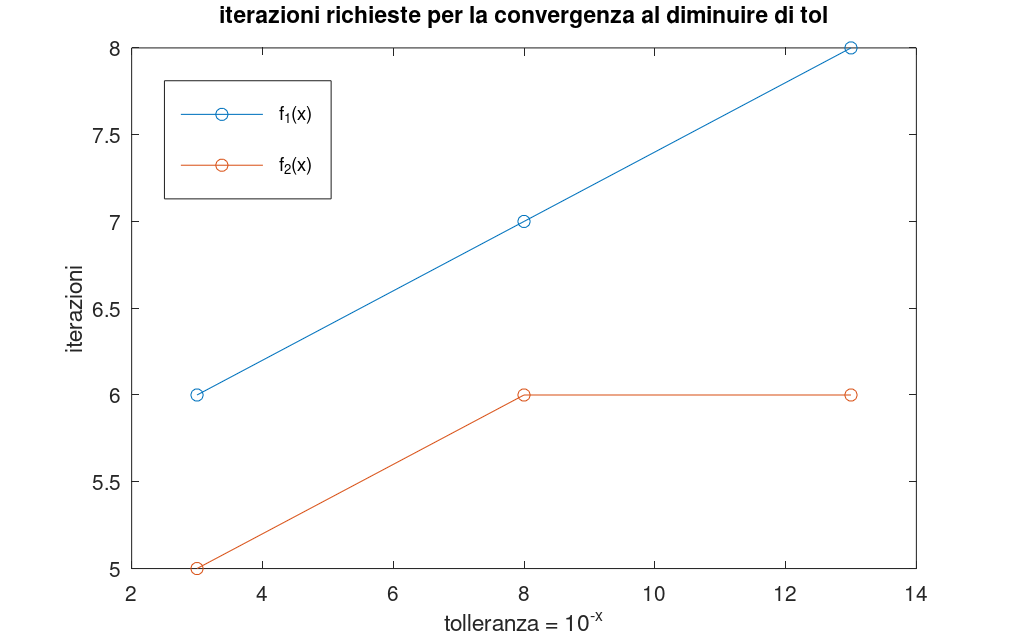
\includegraphics[width=16cm,height=12cm,keepaspectratio]{capitolo4/es15_figure.png}
    \caption{iterazioni richieste}
    \label{fig:es15}
\end{figure}
\newline
Come si vede da risultati ottentui l'accuratezza di funzione di esercizio precedente
rispetta la tolleranza richiesta, quindi criterio di arresto è stato scielto in modo giusto.

Parlando di iterazioni richeiste, si vede, che in funzione con più esponenziali, cioè prima
sono richiesti più iterazioni dato la più alta complessità dei calcoli.
